\section{Muhammad Abdul Gani Wijaya 1174071}
\subsection{Menggunakan library Shapefile dengan Python (pyshp)}
\begin{enumerate}
	\item Nomor 1
	\lstinputlisting{src/tugas2/1174071/soal1.py}
	\begin{figure}[H]
		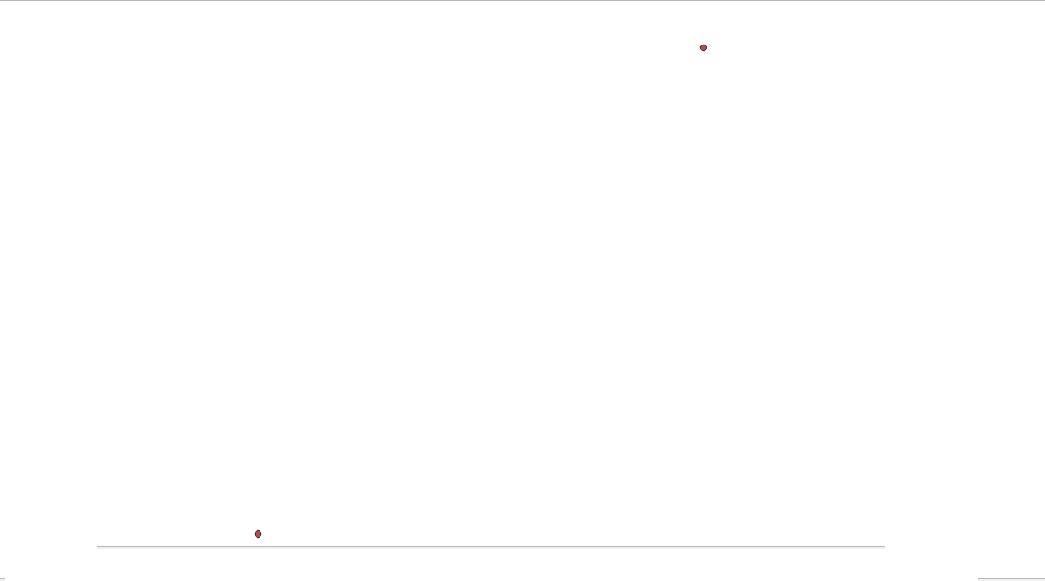
\includegraphics[width=6cm]{figures/Tugas2/1174071/soal1.png}
		\centering
		\caption{Point (Titik)}
	\end{figure}
	\item Nomor 2
	\lstinputlisting{src/tugas2/1174071/soal2.py}
	\begin{figure}[H]
		
\includegraphics[width=6cm]{figures/Tugas2/1174071/soal2.png}
		\centering
		\caption{Point (Titik)}
	\end{figure}
	\item Nomor 3
	\lstinputlisting{src/tugas2/1174071/soal3.py}
	\begin{figure}[H]
		
\includegraphics[width=6cm]{figures/Tugas2/1174071/soal3.png}
		\centering
		\caption{Point (Titik)}
	\end{figure}
	\item Nomor 4
	\lstinputlisting{src/tugas2/1174071/soal4.py}
	\begin{figure}[H]
		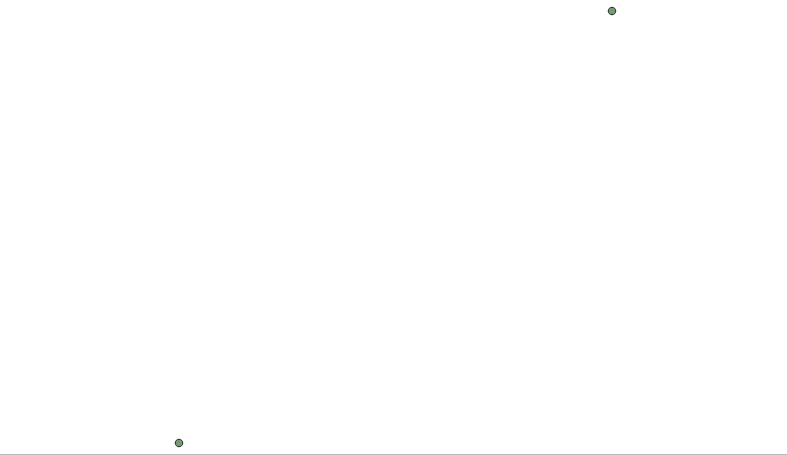
\includegraphics[width=6cm]{figures/Tugas2/1174071/soal4.png}
		\centering
		\caption{Point (Titik)}
	\end{figure}
	\item Nomor 5
	\lstinputlisting{src/tugas2/1174071/soal5.py}
	\begin{figure}[H]
		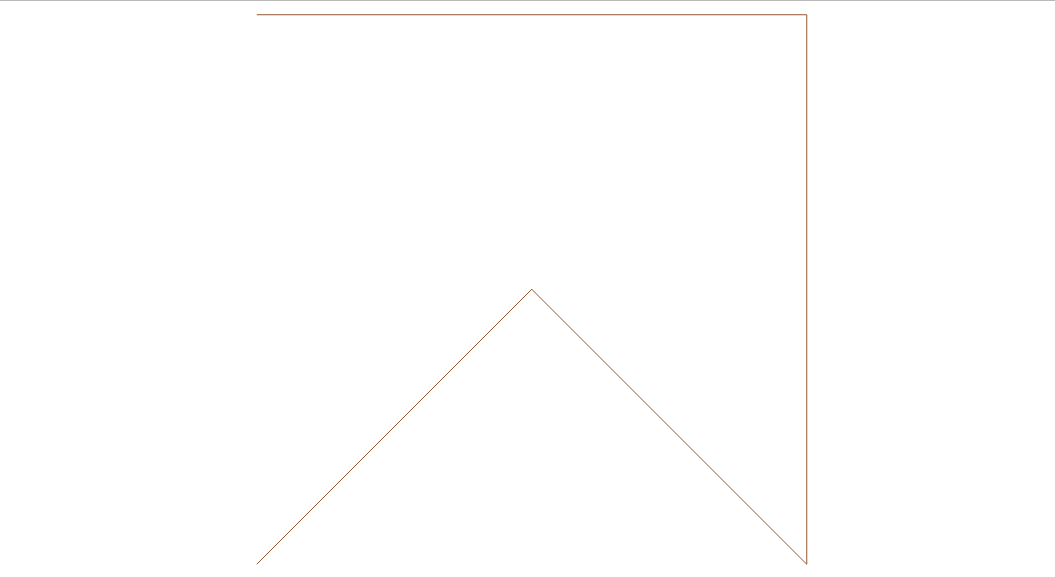
\includegraphics[width=6cm]{figures/Tugas2/1174071/soal5.png}
		\centering
		\caption{PolyLine (Garis)}
	\end{figure}
	\item Nomor 6
	\lstinputlisting{src/tugas2/1174071/soal6.py}
	\begin{figure}[H]
		
\includegraphics[width=6cm]{figures/Tugas2/1174071/soal6.png}
		\centering
		\caption{PolyLine (Garis)}
	\end{figure}
	\item Nomor 7
	\lstinputlisting{src/tugas2/1174071/soal7.py}
	\begin{figure}[H]
		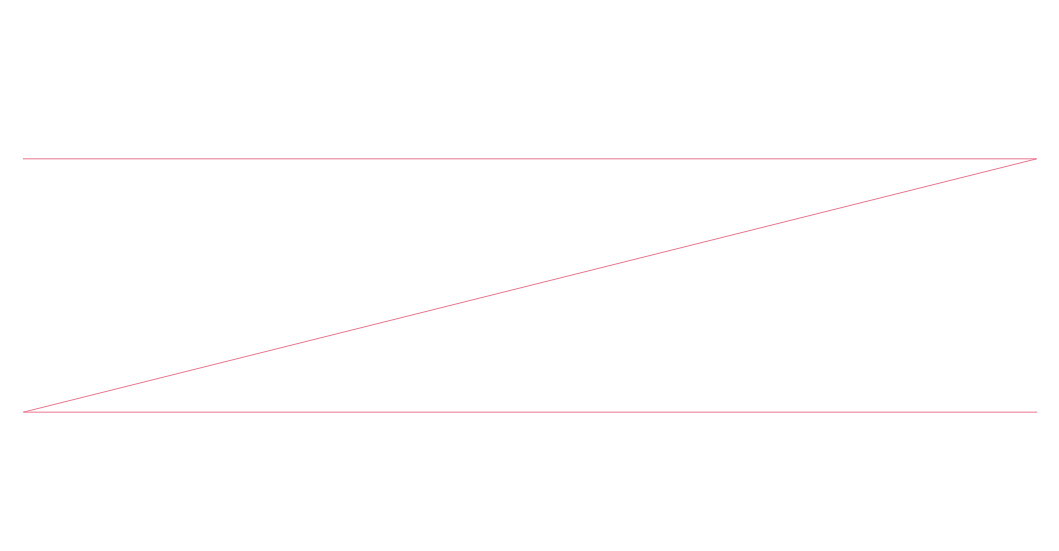
\includegraphics[width=6cm]{figures/Tugas2/1174071/soal7.png}
		\centering
		\caption{Polyline (Garis)}
	\end{figure}
	\item Nomor 8
	\lstinputlisting{src/tugas2/1174071/soal8.py}
	\begin{figure}[H]
		
\includegraphics[width=6cm]{figures/Tugas2/1174071/soal8.png}
		\centering
		\caption{Polygon (Bidang)}
	\end{figure}
	\item Nomor 9
	\lstinputlisting{src/tugas2/1174071/soal9.py}
	\begin{figure}[H]
		
\includegraphics[width=6cm]{figures/Tugas2/1174071/soal9.png}
		\centering
		\caption{Polygon (Bidang)}
	\end{figure}
	\item Nomor 10
	\lstinputlisting{src/tugas2/1174071/soal10.py}
	\begin{figure}[H]
		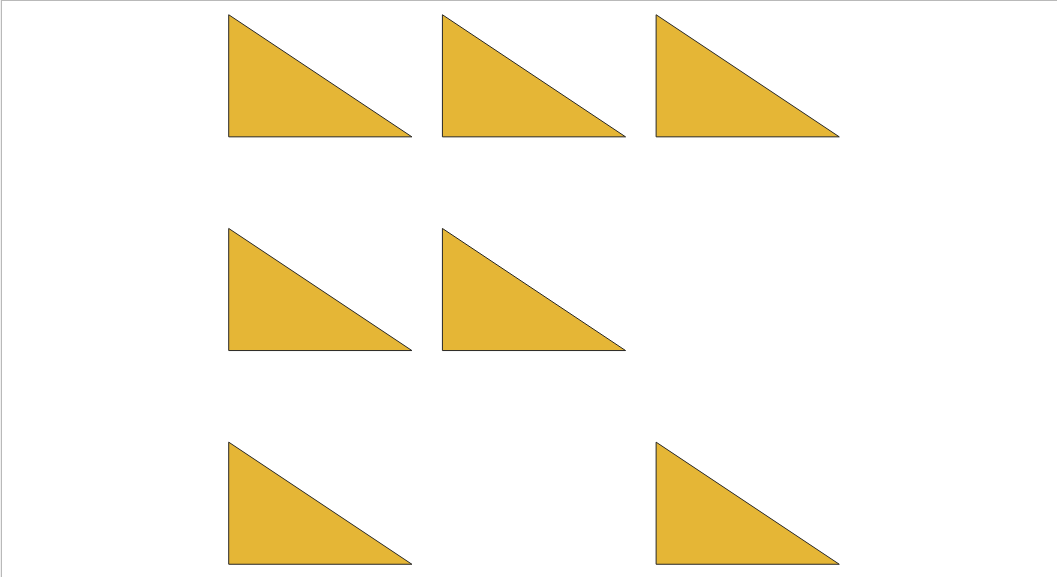
\includegraphics[width=6cm]{figures/Tugas2/1174071/soal10.png}
		\centering
		\caption{Polygon, Hasil modulus dari npm saya 1174071 adalah 7 ,  membuat bangun datar segitiga siku-siku. Angka kedua npm dari belakang adalah 7 sehingga membuat 7 bangun datar segita siku-siku}
	\end{figure}
\end{enumerate}
\subsection{Link Youtube}
https://youtu.be/EozXKmVh-tc